\section{Embedded Context}\label{sec:embedded_context}
Over the years ontologies were used in many domain contexts, including general-purpose as well as highly specialised ones. Obviously, what separates good ontologies from poor ones is how well they are documented~\cite{daquin2012}. Studies~\cite{dutta2017} analysed various approaches of embedding meta-data in ontologies. The outcome was that there is no standard way to describe and document ontologies, albeit a few vocabularies that describe semantic meta-data exist. 

In this section we give an overview of these approaches and explain in detail how we used them for ontology validation. In the remainder of this section our focus lies on semantic meta-data in the context of ontology engineering. A broader discussion on the use of meta-data in general is given in~\cite{nilsson2010}. 

\paragraph{Dublin Core~(DC)}\label{sec:dublin_core_metadata_vocabulary} Being one of the most prominent vocabulary in describing semantic meta-data, published and maintained by the Dublin Core Metadata Initiative~(DCMI), it originally contained 15 meta-data terms\footnote{\url{http://www.dublincore.org/documents/dces/} accessed 2018/05/20},  designed to annotate resources with simple, textual information. Since its first launch, the project have gained popularity, including more than 127 terms\footnote{\url{http://www.dublincore.org/documents/dcmi-terms/} accessed 2018/05/20}. The initial set of terms is listed in~\hyperref[app:dc_terms]{Appendix~\ref*{app:dc_terms}}. 

To maximise interoperability in heterogeneous environments, an RDF-Schema with DCMI-Metadata\footnote{\url{http://dublincore.org/schemas/rdfs/} accessed 2018/05/20} elements was created, in which each entity is identified by a Uniform Resource Identifier~(URI) starting with the prefix \emph{http://purl.org}. 

\paragraph{Simple Knowledge Organisation~(SKOS)} The SKOS Core Vocabulary~\cite{skos2005} defines a set of RDF properties and RDFS classes
used to express the content and structure of a concept scheme, which describes sets of concepts with optionally linked concepts. The vocabulary is standardised by the W3C~Consortium\footnote{\url{https://www.w3.org/TR/skos-reference/} accessed 2018/05/20}. Relevant terms are listed in~\hyperref[app:skos_terms]{Appendix~\ref*{app:skos_terms}}.
	
There is some overlap between DC and SKOS. For example, the terms \textit{dc:subject} and \textit{skos:subject} describes similar characteristics of an entity. However, in some usage scenarios the range of skos:subject is limited to resources of type skos:concept compared to the unrestricted range of dc:subject. Moreover, in case there is more than one subject, the property \textit{skos:primarySubject} allows assertions of the entities or resources main subject. 

\paragraph{Open Biomedical Ontology~(OBO)} Most biomedical ontologies are semantically rich and contain tens of thousands of classes. Managing these is expensive and often requires expert knowledge. The Open Biomedical Ontologies~(OBO)~Foundry\footnote{\url{http://obofoundry.org/} accessed 2018/05/21}, a community of experienced ontology developers and engineers for biomedical environments, manages many specialised biomedical ontologies. These are available in various formats, including the OBO~format, which was originally developed as part of the Gene Ontology~(GO)\footnote{\url{http://www.geneontology.org/} accessed 2018/05/21}. 

The OBO File Format Specification~1.2~\footnote{\url{https://owlcollab.github.io/oboformat/doc/GO.format.obo-1_2.html} accessed 2018/05/22} defines a flat document structure for OBO files. A file contains a header and one or more \emph{stanzas}. A stanza is a labeled section of a document, indicating that an object of a particular type is being described. Currently, there are three supported types: \textit{Term}, \textit{Typedef} and \textit{Instance}. Every stanza starts with an id-tag and an unbounded list of tag-value pairs. Looking at the supported tags, it is clear that the definition of meta-data is important to achieve the goals of \textit{readability}, \textit{ease of parsing}, \textit{extensibility} and \textit{minimal redundancy}. In particular, it allows, among others, the specification of 
\begin{inparaenum}[1)]
		\item the term definition (\texttt{def}),
		\item comments (\texttt{comment}),
		\item editorial data~(\texttt{is\_obsolete}, \texttt{replaced\_by}, \texttt{created\_by}, \texttt{creation\_date}) and
		\item cross references (\texttt{xref})
\end{inparaenum}.

Although the Open Biomedical Ontologies and Semantic Web representation languages have overlapping objectives, they evolved independently. To bring these two communities together, researchers have created a tool for converting OBO~ontologies to OWL and vice-versa without loosing any information during the conversion process~\cite{tirmizi2011}. It turned out that the majority of the OBO~vocabulary fits nicely into the Semantic Web Layer Cake. The mapping between the OBO Layer Cake and the Semantic Web Layer Cake is shown in~\hyperref[fig:semantic_obo_cake]{Figure~\ref*{fig:semantic_obo_cake}}. 

\begin{figure}
	 \centering
	 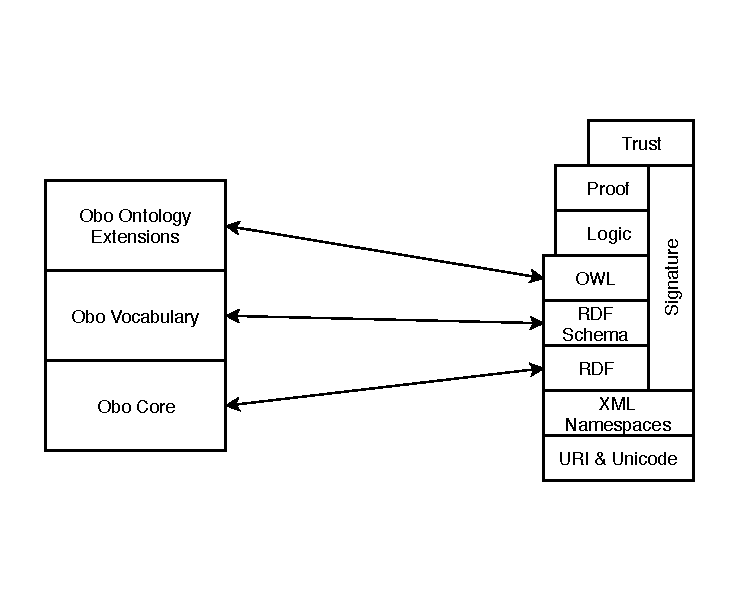
\includegraphics[width=0.5\textwidth]{drawio/Obo2Owl}
	 \caption{Mapping between OBO and the Semantic Web (depicted from~\cite{tirmizi2011})}\label{fig:semantic_obo_cake}
\end{figure}

\emph{OBO~Core} forms the bottom layer of the OBO Layer Cake. It mainly handles the assignment of ids and namespaces to RDF related concepts. Historically, OBO identifiers were limited in scope (local identifiers) while OWL requires global identifiers (URIs). This imposes some challenges on the translation process, e.g. URIs need to be prepended with prefixes. 

The next layer represents the \emph{OBO Vocabulary} which is mapped to RDF-Schema. As there exists a replacement for each of the terms in RDF-Schema, the translation process is implemented by replacing \texttt{names} with RDFS labels, \texttt{definitions} with RDFS labels, \texttt{comments} with RDFS comments, \texttt{is\_a} with subclass relations, \texttt{domains} with RDFS domain restrictions and \texttt{ranges} with RDFS range restrictions. 

The top most layer is represented by the \emph{OBO Ontology Extensions} which are mapped to OWL. Besides the definition of concept-level mappings, this layer defines tags for expressing meta-data on the entire ontology. For example, editorial meta-data (\texttt{creation\_date}, \texttt{replaced\_by} and \texttt{saved\_by}) is mapped to annotation properties. 

A summary of the most important OBO tags together with their OWL equivalents is given in~\hyperref[app:obo_terms]{Appendix~\ref*{app:obo_terms}}. However, for some OBO vocabulary there is no corresponding OWL tag. Therefore, a dedicated OWL namespace\footnote{http://www.geneontology.org/formats/oboInOwl\#} containing all OBO definitions was created. Furthermore, a recommended practice to preserve compatibility between OBO features and OWL features is to restrict editing of mapped OBO tags. A more detailed discussion on this topic is given in~\cite{tirmizi2011, tirmizi2006}.

\paragraph{Meta-Data based Approach}\label{sec:enrichment_metaData_approach}
Given the high number on ontology meta-data formats from above, \hyperref[alg:embedded_enrichment]{Algorithm~\ref*{alg:embedded_enrichment}} shows the pseudocode to create concept descriptions extracted from embedded meta-data. In addition to the notation used in the previous section we define $\Phi(C) \coloneqq \{m_1, m_2, \ldots, m_i \}$ where $m_i$ is the $i'th$ meta-data element embedded in concept $C$ and $T$ is the description of some meta-data element.

\begin{algorithm}
	\caption{Context Enrichment based on embedded meta-data}\label{alg:embedded_enrichment}
	\begin{algorithmic}[1]
		\Procedure{Generate Description}{}\newline
			\textbf{Input:} A concept $C$ with embedded meta-data $\{m_1, m_2, \ldots, m_i \}$\newline
			\textbf{Output:} A description $T$ of $C's$ meta-data elements\newline
			\State{$T=\{\}$}
			\For {$ m_k \in \Phi(C) $}
				\State $T=T$ $\cup$ $m_k$
			\EndFor
		\EndProcedure
	\end{algorithmic}
\end{algorithm}

While the actual enrichment is straightforward, it collects all descriptions for a determined concept, the details of extracting the meta-data from annotation properties is omitted here because it highly depends on the chosen meta-data encoding.
As we decided to encode the meta-data in annotation properties, the extraction process works by selecting the related annotation properties for a specified concept. 
